\documentclass[11pt]{article}
%\usepackage{graphicx}    % needed for including graphics e.g. EPS, PS
\usepackage{setspace}
\usepackage{amsfonts}
\usepackage{amsmath}
\usepackage{amssymb}
\usepackage{enumitem}
\usepackage{longtable}
\usepackage{algpseudocode}
\usepackage{tikz}
\topmargin -1.5cm        % read Lamport p.163
\oddsidemargin -0.04cm   % read Lamport p.163
\evensidemargin -0.04cm  % same as oddsidemargin but for left-hand pages
\textwidth 16.59cm
\textheight 21.94cm
\pagestyle{empty}       % Uncomment if don't want page numbers
\parskip 7.2pt           % sets spacing between paragraphs
\renewcommand{\baselinestretch}{1} % Uncomment for 1.5 spacing between lines
\parindent 0pt         % sets leading space for paragraphs

\begin{document}
\title{COMS 331: Theory of Computing, Fall 2021\\
Semester Notes\\}
\author{Aaron Hanrahan}
\date{}
\maketitle

\section{Alphabets and Strings}

\begin{tabular}{ll}
{\bf Def:} & an \underline{alphabet} is a finite set of objects that we regard as symbols \\
& ex: {0,1}, {a,b} \\
\\
{\bf Def:} & a \underline{string} is over an alphabet \\
& ex: 1101 is a string over {0,1} \\
\\
{\bf Notation:} & $\Sigma^*$ is the set of strings over $\Sigma$ \\
& ex: $\{0,1\}^*$ is the set of binary strings \\
& the \underline{length} of a string $x \in \{0,1\}^*$ is the total number of occurrences of symbols in $x$\\
& ex: $|1101|=4$ \\
\\
{\bf Question:} & What is $\emptyset^*$? \\
{\bf Answer:} & $\emptyset^*=\{\lambda\}$ \\
& Intelligent first answer: $\emptyset^* = \emptyset$ (wrong)\\
& $\Sigma^*=\{a_1,a_2,\cdots,a_n|n \geqslant 0$ and each $a_i\in\Sigma\}$\\
{\bf Further cautions:} & $\{a,b\}=\{b,a\}$, but $ab \neq ba$ (unless $a=b$) \\
& $\{a,a,b\}=\{a,b\}$, but $aab\neq ab$ \\
\\
{\bf Def:} & The \underline{concatenation} of two strings $x,y\in\Sigma^*$ is the string $xy$ \\
& ex: the concatenation of 1101 and 001 is 1101001 \\
& - not an invertable operation, can't ask which strings were concatenated \\
\end{tabular}

\begin{tabular}{ll}
{\bf Properties of Concatenation:} & - Associative: $x(yz)=(xy)z$ \\
& - Identity: $\lambda x = x\lambda$\\
& - Additivity of length: $|xy| = |x| + |y|$\\
& - Not commutative
\end{tabular}

\begin{tabular}{ll}
{\bf Notation:} & for $x\in\Sigma^*$ and $a\in\Sigma$ \\
& $\#(a,x)=\#_a(x)=$ the number of $a$'s in $x$\\
{\bf Def:} & If $x$ and $y$ are strings, then $x$ is a \underline{prefix} of $y$ ($x\sqsubseteq y$),\\ 
& if there exists $z\in\Sigma^*$ such that $xz=y$\\
\\
{\bf Remarks:} & For all $x\in\Sigma^*$, $\lambda \sqsubseteq x$ (because you can take $z=x$), and \\
& $x \sqsubseteq x$ (because can take $z=\lambda$)\\
\end{tabular}

\newpage

\begin{tabular}{ll}
{\bf Def:} & $x$ is a \underline{proper prefix} of $y$ $\Rightarrow$ $x \not\sqsubseteq y$, if $x \sqsubseteq y$ and $x \neq y$\\
\\
{\bf Notation:} & the standard enumeration of $\{0,1\}^*$ is \\
& $\lambda,0,1,00,01,11,000,001,\cdots$\\
& $s_0,s_1,s_2,\cdots$\\
& The natural number represented by a string $x\in\{0,1\}^*$ is the number $\textit{bnum}(x)$\\
& defined by the following recursion: \\
& $\textit{bnum}(\lambda) = 0$ \\
& $\textit{bnum}(x0) = 2\textit{bnum}(x)$ \\
& $\textit{bnum}(x1) = 2\textit{bnum}(x) + 1$
\end{tabular}

\section{Sets}

\begin{tabular}{ll}
{\bf Set Operations:} & If $A$ and $B$ are sets, then \\
& $A \cup B = \{x|x\in A $ or $x \in B\}$ \\
& $A \cap B = \{x|x\in A $ and $x \in B\}$ \\
& $A - B = \{x|x\in A $ and $x \not\in B\}$ \\
& $A \subseteq B$ = every element of $A$ is an element of $B$ \\
& $A \not\subseteq B$ = $A$ is a proper subset of $B$ $\Rightarrow$ $A \subseteq B$ and $A \neq B$\\
\\
{\bf Def:} & A \underline{language} over an alphabet $\Sigma$ is a set of $A \subseteq \Sigma^*$ \\
& ex: The set \\
& PRIMES = $\{x\in\{0,1\}^*|x$ is the binary representation of a prime number$\}$ \\
& is a language over $\{0,1\}$\\
\\
{\bf Def:} & The \underline{concatenation} of two languages $A,B\subseteq\Sigma^*$ is the language \\
& $AB = \{xy|x\in A$ and $y\in B\}$\\
& \underline{Note}: If $A$ and $B$ are finite, then $|AB| \leqslant |A| * |B|$, \\
& has to be $\leqslant$ because there could be repeats. \\
\\
{\bf Def:} & A \underline{prefix set} is a language $A \subseteq \{0,1\}^*$ with the property that no element of $A$ \\
& is a prefix of another element of $A$. \\
& Kraft's inequality proves that this is true. \\
\end{tabular}

\section{Finite Automata and Regular Sets}

\begin{tabular}{ll}
{\bf Def:} & A \underline{deterministic finite automata} (or DFA) is a 5-tuple \\
& $M = (Q,\Sigma,\delta,s,F)$ where \\
& $\cdot$ $Q$ is a finite set whose elements are states \\
& $\cdot$ $\Sigma$ is an alphabet, called the input alphabet \\
& $\cdot$ $s\in Q$ is the start state \\
& $\cdot$ $F \subseteq Q$ is the set of accepting states \\
& $\cdot$ $\delta : Q \times E \rightarrow Q$ is the transition function \\
& The set of strings $L(M)$ accepted by $M$ is a language over $\Sigma$\\
\\
{\bf Example:} & Let $M = (Q,\Sigma,\delta,s,F)$ where $Q=\{0,1,2,3\}$, $\Sigma = \{0,1\}$, $F = \{3\}$ \\
& and $\delta$ is given by the following table: \\
&   \begin{tabular}{c|c|c}
	$\delta(q,a)$ & 0 & 1 \\\hline
	0 & 0 & 1 \\
	1 & 1 & 2 \\
	2 & 2 & 3 \\
	3 & 3 & 3 \\
	\end{tabular} \\
& The DFA can also be represented as: \\
& 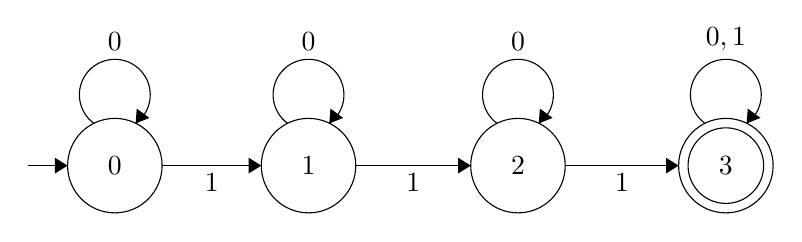
\begin{tikzpicture}[scale=0.2]
\tikzstyle{every node}+=[inner sep=0pt]
\draw [black] (5.7,-9) circle (3);
\draw (5.7,-9) node {$0$};
\draw [black] (18,-9) circle (3);
\draw (18,-9) node {$1$};
\draw [black] (31.3,-9) circle (3);
\draw (31.3,-9) node {$2$};
\draw [black] (44.5,-9) circle (3);
\draw (44.5,-9) node {$3$};
\draw [black] (44.5,-9) circle (2.4);
\draw [black] (0.2,-9) -- (2.7,-9);
\fill [black] (2.7,-9) -- (1.9,-8.5) -- (1.9,-9.5);
\draw [black] (4.377,-6.32) arc (234:-54:2.25);
\draw (5.7,-1.75) node [above] {$0$};
\fill [black] (7.02,-6.32) -- (7.9,-5.97) -- (7.09,-5.38);
\draw [black] (8.7,-9) -- (15,-9);
\fill [black] (15,-9) -- (14.2,-8.5) -- (14.2,-9.5);
\draw (11.85,-9.5) node [below] {$1$};
\draw [black] (16.677,-6.32) arc (234:-54:2.25);
\draw (18,-1.75) node [above] {$0$};
\fill [black] (19.32,-6.32) -- (20.2,-5.97) -- (19.39,-5.38);
\draw [black] (21,-9) -- (28.3,-9);
\fill [black] (28.3,-9) -- (27.5,-8.5) -- (27.5,-9.5);
\draw (24.65,-9.5) node [below] {$1$};
\draw [black] (34.3,-9) -- (41.5,-9);
\fill [black] (41.5,-9) -- (40.7,-8.5) -- (40.7,-9.5);
\draw (37.9,-9.5) node [below] {$1$};
\draw [black] (29.977,-6.32) arc (234:-54:2.25);
\draw (31.3,-1.75) node [above] {$0$};
\fill [black] (32.62,-6.32) -- (33.5,-5.97) -- (32.69,-5.38);
\draw [black] (43.177,-6.32) arc (234:-54:2.25);
\draw (44.5,-1.75) node [above] {$0,1$};
\fill [black] (45.82,-6.32) -- (46.7,-5.97) -- (45.89,-5.38);
\end{tikzpicture} \\
\\
& $M$ accepts the language $L(M)=\{x\in\{0,1\}^*|\#(1,x)\geqslant 3\}$ \\
\\
{\bf Def:} & The \underline{extended transition function} $\hat{\delta}: Q \times \Sigma^* \rightarrow Q$ intuitively defines a path \\
& for an arbitrary string $x$ from $q\in Q$ to $\hat{\delta}(q,x)$. \\
& Formally, $\hat{\delta}$ is defined recursively as follows: \\
& $\cdot$ $\hat{\delta}(q,\lambda)=q$\\
& $\cdot$ For $x\in\Sigma^*$ and $a \in \Sigma$, $\hat{\delta}(q,xa) = \delta(\hat{\delta}(q,x),a)$ \\
\\
{\bf Def:} & Let $M = (Q,\Sigma,\delta,s,F)$ be a DFA, and let $x\in\Sigma^*$,\\
& 1. $M$ accepts $x$ if $\hat{\delta}(s,x)\in F$\\ 
& 2. $M$ rejects $x$ if $\hat{\delta}(s,x)\not\in F$\\ 
& 3. $L(M)=\{x\in\Sigma^*|M$ accepts $x\}$
\end{tabular}

\newpage

\section{Regular Languages}

\begin{tabular}{ll}
{\bf Def:} & A language $A \subseteq \Sigma^*$ is \underline{regular} if there is a DFA $M$ such that $L(M)=A$.\\
\\
{\bf Example:} & Prove that the language $A = \{x\in\{0,1\}^*|$ $3|bnum(x)\}$ \\
& (i.e. num divisible by 3) is regular. \\
& To prove that a language is regular, construct a DFA for it, as seen below: \\
& 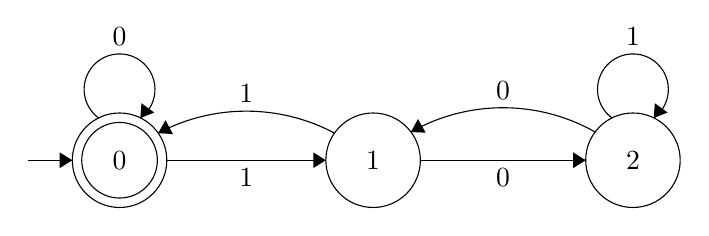
\begin{tikzpicture}[scale=0.2]
\tikzstyle{every node}+=[inner sep=0pt]
\draw [black] (6,-9) circle (3);
\draw (6,-9) node {$0$};
\draw [black] (6,-9) circle (2.4);
\draw [black] (22.1,-9) circle (3);
\draw (22.1,-9) node {$1$};
\draw [black] (38.6,-9) circle (3);
\draw (38.6,-9) node {$2$};
\draw [black] (8.446,-7.277) arc (117.95983:62.04017:11.952);
\fill [black] (8.45,-7.28) -- (9.39,-7.34) -- (8.92,-6.46);
\draw (14.05,-5.38) node [above] {$1$};
\draw [black] (9,-9) -- (19.1,-9);
\fill [black] (19.1,-9) -- (18.3,-8.5) -- (18.3,-9.5);
\draw (14.05,-9.5) node [below] {$1$};
\draw [black] (24.496,-7.209) arc (119.54184:60.45816:11.872);
\fill [black] (24.5,-7.21) -- (25.44,-7.25) -- (24.95,-6.38);
\draw (30.35,-5.17) node [above] {$0$};
\draw [black] (25.1,-9) -- (35.6,-9);
\fill [black] (35.6,-9) -- (34.8,-8.5) -- (34.8,-9.5);
\draw (30.35,-9.5) node [below] {$0$};
\draw [black] (4.677,-6.32) arc (234:-54:2.25);
\draw (6,-1.75) node [above] {$0$};
\fill [black] (7.32,-6.32) -- (8.2,-5.97) -- (7.39,-5.38);
\draw [black] (0.2,-9) -- (3,-9);
\fill [black] (3,-9) -- (2.2,-8.5) -- (2.2,-9.5);
\draw [black] (37.277,-6.32) arc (234:-54:2.25);
\draw (38.6,-1.75) node [above] {$1$};
\fill [black] (39.92,-6.32) -- (40.8,-5.97) -- (39.99,-5.38);
\end{tikzpicture} \\
\\
{\bf Product Construction:} & Let $M = (Q_A\times Q_B, \Sigma, \delta, s, F)$ where \\
& $\delta : (Q_A \times Q_B) \times \Sigma \rightarrow Q_A \times Q_B$  is defined by \\
& $\delta((q,r),a)=(\delta_A(q,a),\delta(r,a))$ for all $q\in Q_A, r \in Q_B,$ and $a \in \Sigma$. \\
& $s=(s_A,s_B)$ and $F=\{(q,r)\in Q_A \times Q_B | q \in F_A$ or $r \in F_B\}$ \\
& for intersection, can use and instead of or for $F$. \\
& \\
& When proving a language is regular, if you can split it up \\
& and prove each part is regular, then you can declare the \\
& combined language regular per the product construction. \\
\end{tabular}

\subsection{Singleton Languages}

\begin{itemize}
\item Given regular languages $A$ and $B$, $A\cup B$, $A\cap B$ and $A$ complements $B$ are all regular. 
\item It is true that every singleton language is regular by problem 16 on homework 3.
\item It is also true that any finite language is regular by problem 17 on homework 3. 
\end{itemize}

{\bf Example 1.} Prove that for all $x\in\Sigma^*$, the singleton language $\{x\}$ is regular.

$\Sigma^*$ is an infinitely long set of $\textit{finite}$ strings. Given any $x\in\Sigma^*$ it is true that $x$ is of finite length. Furthermore, $\{x\}$ is a finite language consisting of a finite string. You can always construct a DFA for a finitely long string, and for every language that you can make a DFA for, it is regular. Therefore, $\{x\}$ is regular. 

{\bf Example 2.} Prove that every finite language $A\subseteq\Sigma^*$ is regular.

A finite language means that it is a finite set of a finite number of inputs (i.e. each input is of finite length). Consider the finite set $Z=\{s_1,s_2,\cdots,s_n\}\subseteq\Sigma^*$. Split $Z$ into singleton languages $Z_1 = \{s_1\}$, $Z_2 = \{s_2\}$, $\cdots$, $Z_n = \{s_n\}$. By the example above, each singleton language $Z_1,Z_2,\cdots,Z_n$ is regular. It is known that the union of two regular languages is a regular language. Therefore, by performing a union on all $Z_1,Z_2,\cdots,Z_n$, this shows that $Z$ is regular. Thus, every finite language is regular. \\

\section{Equivalence Relations}

\subsection{Review of Equivalence Relations}

\begin{itemize}
\item An equivalence relation on a set $X$ is a binary relation $\equiv$ on $X$ that is reflexive, symmetric, and transitive.
\item If $\equiv$ is an equivalence relation on $X$ and $x\in X$, then the $\equiv$ \underline{equivalence class} of $x$ is the set 
$[x]_\equiv = [x]=\{y\in X| x \equiv y\}$
\item If $X$ is a set and $\equiv$ is an equivalence relation on $X$, then the \underline{quotient} of $X$ by $\equiv$ is the set $X/_\equiv=\{[x]_\equiv | x \in X\}$
\item a partition of a set $X$ is a collection $P$ of subsets $B$ of $X$ with properties:
\begin{itemize}
\item each element of $P$ is nonempty
\item $\bigcup\limits_{B\in P} B = X$
\item For all $B_1, B_2 \in P, B_1 \neq B_2 \Rightarrow B_1 \cap B_2 = \emptyset$
\end{itemize}
\end{itemize}

\subsection{Fundamental Theorem of Equivalence Relations}

\begin{tabular}{ll}
& Let $X$ be a set. \\
1. & For every equivalence relation $\equiv$ on $X$, $X/_\equiv$ is a partition of $X$. \\
2. & For every partition $P$ of $X$, the relation $\equiv$ on $X$ defined by $x\equiv y$ if and only if \\
& there exists a $B\in P $ such that $x,y\in B$.
\end{tabular}

\begin{tabular}{ll}
{\bf Def:} & If $\equiv$ is an equivalence relation on a set $S$, then a set $A \subseteq S$ \underline{respects} $\equiv$ \\
& if for all $x,y\in S$, $x \equiv y \Rightarrow [x\in A$ $\textit{iff}$ $y\in A]$ \\
\\
{\bf Obs:} & If $\equiv$ is an equivalence relation on a set $S$, then $\forall A \subseteq S$, \\
& the following conditions are equivalent: \\
& (1) $A$ respects $\equiv$ \\
& (2) There is a set $I\subseteq{S/_\equiv}$ such that $A=\bigcup\limits_{C\in I}C$\\
\\
{\bf Def:} & For a DFA $M=(Q,\Sigma ,\delta ,s, F)$, define the relation $\equiv_M$ on $\Sigma^*$ by \\
& $x\equiv_M y$ $\textit{iff}$ $\hat{\delta}(s,x)=\hat{\delta}(s,y)$
\end{tabular}

\begin{tabular}{ll}
{\bf Observation 1:} & For each $q\in Q$, let $C_{m,q} = \{x\in\Sigma^*|\hat{\delta}(s,x)=q\}$ \\
& Define a state $q\in Q$ to be \underline{reachable} in $M$ if $C_{m,q}\neq\emptyset$.\\
& Otherwise, $q$ is unreachable in $M$. \\
{\bf Observation 2:} & An equivalence class $\equiv$ on a set $S$ has \underline{finite index} if \\
& $|S/_\equiv < \infty$, i.e. if it has only finitely many equivalence classes. \\
& Otherwise, $\equiv$ has infinite index. \\
{\bf Observation 3:} & For every DFA $M$, the equivalence relation $\equiv_M$ has finite index.\\
& An equivalence relation $\equiv$ is \underline{right-invariant} if, for all $x,y,z\in\Sigma^*$\\
& $x \equiv y \Rightarrow xz \equiv yz$.\\
{\bf Observation 4:} & For every DFA $M$, $\equiv_M$ is right-invariant.\\
{\bf Observation 5:} & For every DFA $M$, $L(M)=\bigcup\limits_{q\in F}C_{m,q}$.\\
\\
{\bf Note:} & Observations 2 and 5 tell us that $L(M)$ respects $\equiv_M$. Taken together, \\
& observations 1-5 tell us that every regular language $A\subseteq\Sigma^*$ respects \\
& a right-invariant equivalence relation of finite index on $\Sigma^*$, namely the relation \\
& $\equiv_M$, where $M$ is any DFA deciding $A$.\\
\\
{\bf Def:} & The \underline{canonical equivalence relation} of a language $A\subseteq\Sigma^*$\\
& is the relation $\equiv_A$ on $\Sigma^*$ defined by: \\
& $x \equiv_A y$ $\textit{iff}$ for all $z \in \Sigma^*$, $xy\in A \Leftrightarrow yz \in A$, i.e., if you can attach \\
& a $z$ to $x,y$ that can distinguish $x,y$, you cannot decide the language. \\
\\
{\bf Observation 6:} & For every language $A\subseteq\Sigma^*$, $\equiv_A$ is a right-invariant equivalence relation on $\Sigma^*$ \\
\\
{\bf Def:} & If $\equiv$ and $\approx$ are equivalence relations on a set $S$, then $\equiv$ \underline{refines} $\approx$ if, \\
& $\forall x,y \in S, x \equiv y \Rightarrow x \approx y$. \\
\\
\end{tabular}

\begin{tabular}{ll}
{\bf Remarks:} & - every equivalence relation defines itself \\
& - every equivalence relation refines $\forall x,y, x \approx y$ \\
& - equality refines every equivalence relation \\
\\
{\bf Observation 7:} & Let $\equiv$ and $\approx$ be equivalence relations on $S$. If $\equiv$ refines $\approx$,\\
& $\equiv$ has finite index $\Rightarrow$ $\approx$ has finite index. \\
{\bf Lemma 8:} & Let $A\subseteq\Sigma^*$, and let $\equiv$ be a right-invariant equivalence relation on $\Sigma^*$,\\
& The following conditions are equivalent: \\
& (1) A respects $\equiv$ \\
& (2) $\equiv$ refines $\equiv_A$ \\
\end{tabular}

\section{Proving Languages Not Regular}

\subsection{Myhill-Nerode}
\begin{tabular}{ll}
{\bf Theorem 9:} & For every language $A \subseteq \Sigma^*$, the following conditions are equivalent:\\
& (1) $A$ is regular \\
& (2) The relation $\equiv_A$ has finite index. \\
& (3) $A$ respects some right-invariant equivalence relation of finite index on $\Sigma^*$ \\
\\
& The Myhill-Nerode relation for $A$ satisfies:\\
& (1) $x\equiv y\Rightarrow xa \equiv ya$ for $x,y\in\Sigma^*$ and $a\in\Sigma$ \\ 
& (2) $x\equiv y \Rightarrow (x\in A \Leftrightarrow y \in A)$ \\ 
& (3) $\equiv$ is of finite index. \\
& (4) Let $M$ be a DFA with no inaccessible states. $x \equiv_M y \Leftrightarrow \hat{\delta}(s,x)=\hat{\delta}(s,y)$\\
\\
{\bf Example:} & The language $A = \{0^n1^n|n\in\mathbb{N}\}$ is not regular. Proof: \\
& Let $A$ be as given. It suffices by Myhill-Nerode to prove that $\equiv_A$ has infinite index. \\
& Let $m,n\in\mathbb{N}$. Since $0^m1^m\in A$ and $0^n1^n \not\in A$, and $A$ respects $\equiv_A$, \\
& it must be the case that $O^m1^m\not\equiv_A 0^n1^m$. Since $\equiv_A$ is right-invariant, \\
& it follows that $0^m\not\equiv 0^n$. Thus, $\equiv_A$ does not have finite index.\\
\end{tabular}

\subsection{Ordinal Extensions}

\begin{itemize}
\item For each set $A\in\Sigma^*$ and each $j\in\mathbb{Z}^+$ not exceeding $|A|$, the $j$th element of $A$ is thus unambiguously defined. 
\item For each $A\subseteq\Sigma^*$ and $x\in\Sigma^*$, let $A_x =\{y\in\Sigma^*|xy\in A\}$ be the set of all \underline{A-extensions} of $x$. $A_x$ is the set of all strings you can add to $x$ and still be in $A$.
\item Define the set $A_x^{(j)}$ as follows:
\begin{itemize}
\item If $j\leqslant |A|$, then $A_x^{(j)}=\{y\}$, where $y$ is the $j$th A-extension of $x$.
\item If $j>|A|$, then $A_x^{(j)}=\emptyset$
\item Note that $|A_x^{(j)}|\leqslant 1$ in any case.
\end{itemize}
\item For each $A,B\subseteq\Sigma^*$ and $j\in\mathbb{Z}^+$, let $A_B^{(j)} = \bigcup\limits_{x\in B}A_x^{(j)}$ be the set of all $j$th extensions of elements of $B$, and let $A^{(j)}=A_{\Sigma^*}^{(j)}$ be the set of all $j$th A-extensions.
\end{itemize}

{\bf Example.} Prove that the language $\{0^k1^m0^n\mid n=k+m\}$ is not regular.

%Problem 37
$Let A = \{0^k1^m0^n\mid n=k+m\}$, and $k=m=p$, $p\in\mathbb{N}$. Let $n=2p$. Consider an $x$ s.t. $x=0^p1^p$, and the first extension of $x$ is $xA^{1}_{x}\in A$. \\
Then consider $y$ s.t. $y=0^{2p}$, and concur that $xy\in{A}$ is accepted. It is true that for every $p$, there is one $y$, and $y$ is dependent on $p$. Because $p$ is infinite, $y$ is also infinite. Then, $|y|=|A^{1}_{x}|=\infty$, showing that $A$ is not regular. \\

\subsubsection{Terminology}

\begin{tabular}{ll}
{\bf Def:} & A language $A\subseteq\Sigma^*$ has \underline{bounded ordinal extensions} if there exists $m\in\mathbb{Z}^+$ such that, \\
& for all $j\in\mathbb{Z}^+$, $|A^{(j)}|\leqslant m$. Otherwise, $A$ has \underline{unbounded ordinal extensions}. \\
\\
{\bf Def:} & A language $A$ has \underline{infinite ordinal extensions} if there exists $j\in\mathbb{Z}^+$ such that $|A^{(j)}|=\infty$. \\
& Clearly, a language with infinite ordinal extensions must have unbounded ordinal extensions. \\
\\
{\bf Example:} & $A=\{0^n1^n|n\in\mathbb{N}\}$ is not regular. Proof:\\
& For each $n\in\mathbb{N}$, $1^n\in A^{(1)}$, because $1^n$ is the first A-extension of $0^n$.\\
\\
{\bf Theorem:} & Every regular language has bounded ordinal extensions. \\
& $\therefore$ To prove that $A$ is not regular, it suffices to show that $A$ has unbounded ordinal extensions. \\
& $\therefore$ For this, it suffices to show that $A$ has infinite ordinal extensions. \\
\\
{\bf Theorem:} & If $A$ has unbounded ordinal extensions, then $A$ is not regular. \\
\\
{\bf Lemma:} & Let $\approx$ be a right-invariant equivalence relation on $\Sigma^*$, and let $A\subseteq\Sigma^*$. \\
& If $A$ respects $\approx$, then $\forall j \in\mathbb{Z}$, $|A^{(j)}| \leqslant |\Sigma^*/_\approx$. 
\end{tabular}

\section{Computability}

\subsection{Turing Machines}

\begin{tabular}{ll}
{\bf Def:} & Per the Church-Turing thesis, a function is computable if and only if there is \\
& a Turing machine that computes it. \\
\\
{\bf Def:} & A \underline{Turing machine} TM is a 9-tuple $M=(Q,\Sigma,\Gamma,\vdash,\square,\delta,s,t,r)$ \\
& $Q$ a finite set of states \\
& $\vdash$ is the left end marker \\
& $\square$ is the empty cell \\
& $\delta : Q \times \Gamma \rightarrow Q \times \Gamma \times \{L,R\}$ \\
& $\Sigma \cup \{\vdash,\square\} \subseteq \Gamma$, and no transition changes $\vdash$ \\
& For all $a\in\Gamma$, $\delta(t,a) = (t,a,R)$ and $\delta(r,a) = (r,a,R)$, i.e. \\
& whether it accepts/rejects, goes endlessly anyways. \\
\end{tabular}

{\bf Example.} Give the formal description for a Turing machine that accepts the language
\begin{center}
    $\{x\mid  \text{the } \#(1,x) \text{-th symbol of }x \text{ is 1}\}$
\end{center}
with $\Sigma=\{0,1\}$.\\

Let $\Gamma = \Sigma \cup \{\vdash, \textvisiblespace,\#,1^*,\not{1},\not{1^*},\not{0}\}$ \\

Intuition (informal description): \\
Read until first blank, replace with \# \\
Go back to beginning ($\vdash$) \\
(1) Go right until reach a 1 \\
\hspace*{8mm} When reach a 1, change the 1 to $1^*$ \\
\hspace*{8mm} Go to first $\textvisiblespace$ after \#, change to a 1 \\
\hspace*{8mm} Go back to last $1^*$ \\
\hspace*{8mm} Repeat (1) \\
Go right until \# (have covered all the original ones by now) \\
Go right to first 1 after \# \\
\hspace*{8mm} Change to $\not{1}$ \\
\hspace*{8mm} Go back to start symbol or last canceled symbol \\
After canceling all 1's, go to last canceled and accept if one, reject if not. \\
\\
Formal description: \\
\begin{center}
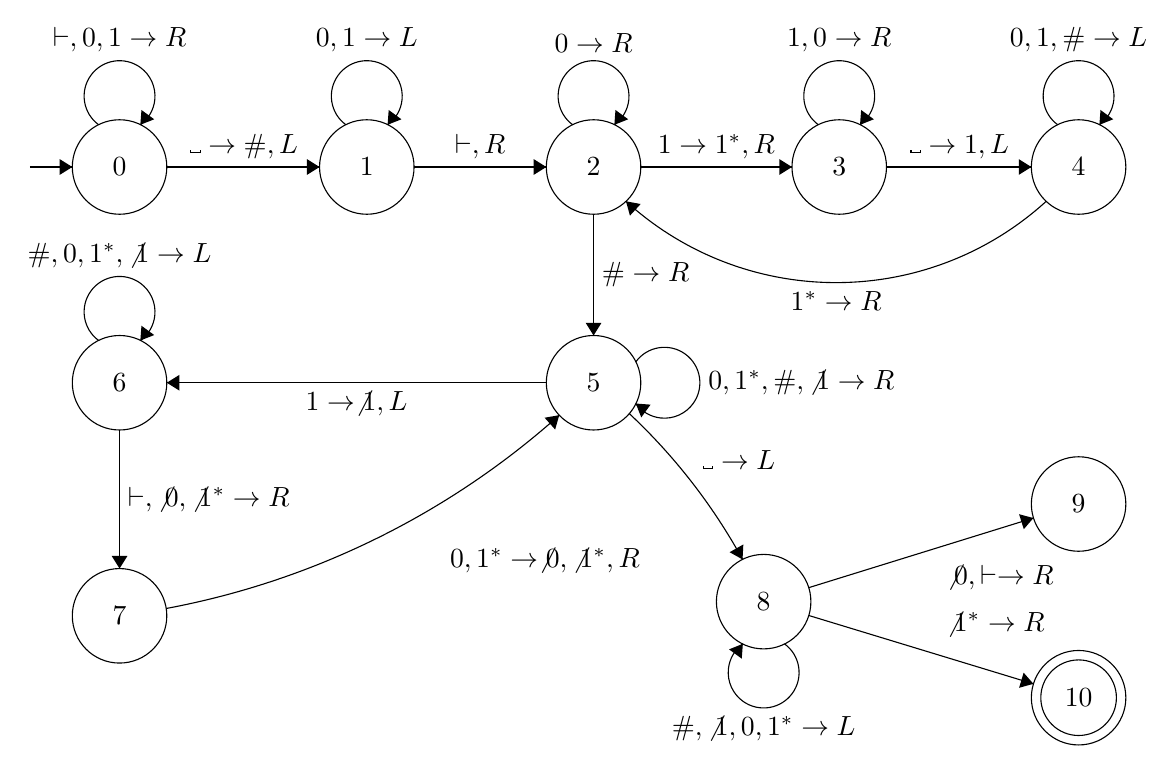
\begin{tikzpicture}[scale=0.2]
\tikzstyle{every node}+=[inner sep=0pt]
\draw [black] (5.9,-9.1) circle (3);
\draw (5.9,-9.1) node {$0$};
\draw [black] (21.6,-9.1) circle (3);
\draw (21.6,-9.1) node {$1$};
\draw [black] (36,-9.1) circle (3);
\draw (36,-9.1) node {$2$};
\draw [black] (51.6,-9.1) circle (3);
\draw (51.6,-9.1) node {$3$};
\draw [black] (66.8,-9.1) circle (3);
\draw (66.8,-9.1) node {$4$};
\draw [black] (36,-22.8) circle (3);
\draw (36,-22.8) node {$5$};
\draw [black] (5.9,-22.8) circle (3);
\draw (5.9,-22.8) node {$6$};
\draw [black] (5.9,-37.6) circle (3);
\draw (5.9,-37.6) node {$7$};
\draw [black] (46.8,-36.7) circle (3);
\draw (46.8,-36.7) node {$8$};
\draw [black] (66.8,-30.5) circle (3);
\draw (66.8,-30.5) node {$9$};
\draw [black] (66.8,-42.8) circle (3);
\draw (66.8,-42.8) node {$10$};
\draw [black] (66.8,-42.8) circle (2.4);
\draw [black] (4.577,-6.42) arc (234:-54:2.25);
\draw (5.9,-1.85) node [above] {$\vdash,0,1\rightarrow R$};
\fill [black] (7.22,-6.42) -- (8.1,-6.07) -- (7.29,-5.48);
\draw [black] (0.2,-9.1) -- (2.9,-9.1);
\fill [black] (2.9,-9.1) -- (2.1,-8.6) -- (2.1,-9.6);
\draw [black] (8.9,-9.1) -- (18.6,-9.1);
\fill [black] (18.6,-9.1) -- (17.8,-8.6) -- (17.8,-9.6);
\draw (13.75,-8.6) node [above] {$\textvisiblespace\rightarrow \#,L$};
\draw [black] (20.277,-6.42) arc (234:-54:2.25);
\draw (21.6,-1.85) node [above] {$0,1\rightarrow L$};
\fill [black] (22.92,-6.42) -- (23.8,-6.07) -- (22.99,-5.48);
\draw [black] (24.6,-9.1) -- (33,-9.1);
\fill [black] (33,-9.1) -- (32.2,-8.6) -- (32.2,-9.6);
\draw (28.8,-8.6) node [above] {$\vdash ,R$};
\draw [black] (34.677,-6.42) arc (234:-54:2.25);
\draw (36,-1.85) node [above] {$0\rightarrow R$};
\fill [black] (37.32,-6.42) -- (38.2,-6.07) -- (37.39,-5.48);
\draw [black] (39,-9.1) -- (48.6,-9.1);
\fill [black] (48.6,-9.1) -- (47.8,-8.6) -- (47.8,-9.6);
\draw (43.8,-8.6) node [above] {$1\rightarrow 1^*,R$};
\draw [black] (50.277,-6.42) arc (234:-54:2.25);
\draw (51.6,-1.85) node [above] {$1,0\rightarrow R$};
\fill [black] (52.92,-6.42) -- (53.8,-6.07) -- (52.99,-5.48);
\draw [black] (54.6,-9.1) -- (63.8,-9.1);
\fill [black] (63.8,-9.1) -- (63,-8.6) -- (63,-9.6);
\draw (59.2,-8.6) node [above] {$\textvisiblespace\rightarrow 1,L$};
\draw [black] (65.477,-6.42) arc (234:-54:2.25);
\draw (66.8,-1.85) node [above] {$0,1,\#\rightarrow L$};
\fill [black] (68.12,-6.42) -- (69,-6.07) -- (68.19,-5.48);
\draw [black] (64.742,-11.279) arc (-47.69169:-132.30831:19.822);
\fill [black] (38.06,-11.28) -- (38.31,-12.19) -- (38.99,-11.45);
\draw (51.4,-16.94) node [below] {$1^*\rightarrow R$};
\draw [black] (36,-12.1) -- (36,-19.8);
\fill [black] (36,-19.8) -- (36.5,-19) -- (35.5,-19);
\draw (36.5,-15.95) node [right] {$\#\rightarrow R$};
\draw [black] (33,-22.8) -- (8.9,-22.8);
\fill [black] (8.9,-22.8) -- (9.7,-23.3) -- (9.7,-22.3);
\draw (20.95,-23.3) node [below] {$1\rightarrow\not{1},L$};
\draw [black] (4.577,-20.12) arc (234:-54:2.25);
\draw (5.9,-15.55) node [above] {$\#,0,1^*,\not{1}\rightarrow L$};
\fill [black] (7.22,-20.12) -- (8.1,-19.77) -- (7.29,-19.18);
\draw [black] (5.9,-25.8) -- (5.9,-34.6);
\fill [black] (5.9,-34.6) -- (6.4,-33.8) -- (5.4,-33.8);
\draw (6.4,-30.2) node [right] {$\vdash,\not{0},\not{1^*}\rightarrow R$};
\draw [black] (33.822,-24.862) arc (-48.22211:-79.41172:51.729);
\fill [black] (33.82,-24.86) -- (32.89,-25.02) -- (33.56,-25.77);
\draw (32.91,-33.26) node [below] {$0,1^*\rightarrow\not{0},\not{1^*},R$};
\draw [black] (38.68,-21.477) arc (144:-144:2.25);
\draw (43.25,-22.8) node [right] {$0,1^*,\#,\not{1}\rightarrow R$};
\fill [black] (38.68,-24.12) -- (39.03,-25) -- (39.62,-24.19);
\draw [black] (38.27,-24.76) arc (46.88883:28.80404:37.29);
\fill [black] (45.46,-34.02) -- (45.51,-33.07) -- (44.64,-33.56);
\draw (42.8,-27.69) node [right] {$\textvisiblespace\rightarrow L$};
\draw [black] (48.123,-39.38) arc (54:-234:2.25);
\draw (46.8,-43.95) node [below] {$\#,\not{1},0,1^*\rightarrow L$};
\fill [black] (45.48,-39.38) -- (44.6,-39.73) -- (45.41,-40.32);
\draw [black] (49.67,-35.81) -- (63.93,-31.39);
\fill [black] (63.93,-31.39) -- (63.02,-31.15) -- (63.32,-32.1);
\draw (61.81,-34.36) node [below] {$\not{0},\vdash\rightarrow R$};
\draw [black] (49.67,-37.58) -- (63.93,-41.92);
\fill [black] (63.93,-41.92) -- (63.31,-41.21) -- (63.02,-42.17);
\draw (61.52,-38.99) node [above] {$\not{1^*}\rightarrow R$};
\end{tikzpicture}
\end{center}


Five methods for proving a language not regular. \\
(1) Brute force: Find inequivalent x,y that DFA must confuse \\
(2) Myhill-Nerode \\
(3) Pumping Lemma \\
(4) Kolmogorov Complexity \\
(5) Ordinal Extensions \\
\\
In principle, (1) and (2) always work with extra ad hoc cleverness. \\
(3), (4), (5) are systematic, and \underline{usually} work. \\
(5) short easy proofs. \\
(4) intuitive (talks about information) 

\subsection{Two string-pairing functions}
$\langle x,y \rangle = 0^{|x|}1xy$ \\
$\langle x,y \rangle = bd(x)01y$, where $bd(1101)=11110011$ (bit double) 

\subsection{Cantor space}
$P(\{0,1\}^*)=\{$languages over alphabet $\{0,1\}\}$ \\
$\{0,1\}^* = \{s_0, s_1, s_2,\cdots\}$ \\
$A \subseteq \{0,1\}^* = \{s_0, s_1, s_2, \cdots\}$ \\
$x_A \in \{0,1\}^{\infty} =$ 0 1 1 0 1 (bitmap of decisions made in $A$ (no, yes, yes, no, yes, $\cdots$) \\

\subsection{Reductions}

\begin{tabular}{ll}
{\bf Def:} & Let $A,B\subseteq\{0,1\}^*$. A \underline{many-one reduction} (a.k.a. m-reduction, or $\leqslant_m$-reduction) \\
& of $A$ to $B$ is a computable function $f:\{0,1\}^*\rightarrow\{0,1\}^*$ s.t. for all $x\in\{0,1\}^*$, \\
& $x\in A \Leftrightarrow f(x)\in B$. \\
\\
& - We say that $A$ is $\leqslant_m$-reducible to $B$, and we write $A\leqslant_m B$ if there exists \\
& $\leqslant_m$-reduction $f$ of $A$ to $B$ \\
\\
\end{tabular}
\\
\begin{tabular}{ll}
{\bf Reducibilities:} & $\leqslant_T$ Turing reducibilities \\
& $\leqslant_m$ \\
& $\leqslant^p_T$ polynomial time Turing reducibility \\
& $\leqslant^p_m$ polnomial $\leqslant_m$
\end{tabular}

\subsection{Decidability and Computability}

\begin{longtable}{ll}
{\bf Def:} & A language $A \subseteq\Sigma ^*$ is \underline{decidable} if there is a TM that (halts on every input and) \\
& decides $A$. \\
\\
{\bf Def:} & A function $f:\{0,1\}^*\rightarrow\{0,1\}^*$ is \underline{computable} if there is a TM that computes it. \\
\\
{\bf Def:} & A \underline{partial function} $f:\subseteq\{0,1\}^*\rightarrow\{0,1\}^*$ is computable if there is a TM that define it. \\
& It might not be defined on all inputs. \\
\\
{\bf Def:} & For each $i\in\mathbb{N}$, the $i$-th TM is the TM $M_i$ s.t. $\#(M_i)=u_i$, then \\
& $M_0, M_1, M_2, \cdots$ is the \underline{standard enumeration of all TMs} \\
& $\textbf{Note}$ that a minor variant of $U$, say $\hat{U}$, has the property that \\
& $\forall(i\in\mathbb{N}\wedge x\in\{0,1\}^*)$, $\hat{U}(\langle i,x \rangle)\cong M_i(x)$ \\
\\
{\bf Notation:} & $\phi_i\subseteq\{0,1\}^*\rightarrow\{0,1\}^*$ is the partial-function computed by $M_i$, then \\
& $\phi_0,\phi_1,\phi_2,\cdots$ is the standard enumeration of all computable partial functions. \\
\\
{\bf Notation:} & $M(x)\downarrow$, $M$ halts on input $x$, $M(x)\uparrow$, $M$ doesn't halt on input. \\
\\
{\bf Def:} & The \underline{rapidly growing function} (Note: max $\emptyset$=0) $G:\mathbb{N}\rightarrow\mathbb{N}$, is defined by \\
& $G(N) = 1 + max\{\phi_k(l)$ s.t. $0 \leqslant k \leqslant n$, $0 \leqslant l \leqslant n$, and $\phi_k(l)\downarrow\}$ \\
\\
{\bf Observation 1:} & $G$ is \underline{total}, i.e., $G(n)$ is defined for all $n$. \\
\\
{\bf Observation 2:} & $G$ is non-decreasing, i.e., $G(n) \leqslant G(n+1)$ for all $n$. \\
\\
{\bf Def:} & The \underline{halting problem} is the set $H=\{(k,l)\in\mathbb{N}\times\mathbb{N}|M_k(l)\downarrow\}$ \\
\\
{\bf Observation 3:} & If $H$ is undecidable, then $G$ is computable. \\
\\
{\bf Lemma 4:} & $G$ grows faster than any computable function. That is, for every \\
& computable function $f:\mathbb{N}\rightarrow\mathbb{N}$, we have $G(n)>f(n)$ for all but \\
& infinitely many $n$. \\
\\
{\bf Corollary 5:} & $G$ is not computable. \\
\\
{\bf Theorem 6:} & $H$ is undecidable. \\
\\
{\bf Lemma 4 Proof:} & Let $f:\mathbb{N}\rightarrow\mathbb{N}$ be computable. Then, there is an index $i\in\mathbb{N}$ s.t. \\
& $\phi_i = f$. Then, for all $n\geqslant i$, $G(n)$ is defined as previously, \\
& $n \geqslant i \Rightarrow \phi_i(n)$ is in the $G(n)$ table. \\
& \begin{tabular}{ccc}
$G(n)$ & $\geqslant$ & 1 + $\phi_i(n)$ \\
& $>$ & $\phi_i(n)$ \\
& = & $f(n)$ $\square$
\end{tabular} \\
\\
{\bf Note:} & Once you know that the halting problem $H$ is undecidable, you usually \\
& prove that other languages $A$ are undecidable by proving that $H \leqslant_m A$. \\
\\
{\bf Def:} & A language $A\subseteq\{0,1\}$ is computable enumerable (CE) if \\
& there is a TM $M$ s.t. $L(M)=A$ where $L(M)$ is the set of all strings accepted \\
& by $M$ ($M$ is not required to halt on strings not in $A$) \\
\\
{\bf Def:} & A language $A\subseteq \{0,1\}^*$ is \underline{co-computably enumerable} (co-CE) if $\{0,1\}^*-A$ is CE \\
& (i.e. the complement of $A$ is CE) \\
\\
& The classes DEC (decidable), CE, and co-CE are defined in the now-obvious ways: \\
& DEC $\subseteq$ CE \\
& $H$ $\in$ CE - DEC ($H$ is in CE, not decidable) \\
& co-DEC = DEC \\
& DEC $\subseteq$ co-CE \\
& $\mathcal{C} \subseteq \mathcal{D} = $co-$\mathcal{C} \subseteq$ co-$\mathcal{D}$, where $\mathcal{C},\mathcal{D}$ are classes \\
& CE $\cap$ co-CE = DEC \\
\\
{\bf Fact:} & For every language $A\subseteq\{0,1\}^*$, the following conditions are equivalent: \\
& (1) $A$ is CE \\
& (2) There is a DEC language $B\subseteq\{0,1\}^*$ s.t. for all $x\in\{0,1\}^*$, \\
& $x\in A \Leftrightarrow (\exists w \in \{0,1\}^*)\langle x,w \rangle \in B$ \\
& (3) There is a CE language $B\subseteq\{0,1\}^*$ s.t. for all $x\in\{0,1\}^*$, \\
& $x\in A \Leftrightarrow (\exists w \in \{0,1\}^*)\langle x,w \rangle \in B$ \\
\\
{\bf Fact:} & CE is \underline{close (downward)} under $\leqslant_m$, meaning that $A \leqslant_m B \subseteq$ CE $\Rightarrow A \in$ CE. \\
& DEC, and co-CE are also closed in this manner. \\
\\
{\bf Def:} & Languages $A,B\in\{0,1\}^*$ are $\leqslant_m$-\underline{equivalent}, and we write $A \equiv_m B$, if \\
& $A \leqslant_m B$ and $B \leqslant_m A$. \\
& Equivalence classes of $\equiv_m$ are called $\equiv_m$-\underline{degrees}. \\
\\
{\bf Def:} & Let $A \subseteq \{0,1\}^*$ be a language, and let $\mathcal{C}$ be a class of languages. \\  
& (1) $A$ is $\leqslant_m$-hard for $\mathcal{C}$ if, for ever $B\in\mathcal{C}$, $\mathcal{C}$. \\
& (at least as hard as anything in $\mathcal{C}$ w/ respect to this reducibility) \\
& (2) $A$ is $\leqslant_m$-complete for $\mathcal{C}$ if $A \in \mathcal{C}$ and $A$ is $\leqslant_m$-hard for $\mathcal{C}$. \\
\\
{\bf Corollary:} & Recall that the halting problem $H=\{(k,l)\in N\times N|M_k(l)\downarrow\}$ is CE. \\
& $H$ is not co-CE. \\
\\
{\bf Theorem:} & $H$ is $\leqslant_m$-complete for $\mathcal{C}$. \\
\\
{\bf Def:} & An \underline{input/output property} of TMs is a set $I \in \mathbb{N}$ s.t., for all \\
& $i,j \in \mathbb{N}$, $\phi_i = \phi_j \Rightarrow [i\in I \Leftrightarrow j \in I]$ \\
\end{longtable}

An I/O property $I$ of TMs is trivial if $I = \emptyset$ or $I = \mathbb{N}$. Otherwise, $I$ is non-trivial. \\

\begin{tabular}{ll}
{\bf Theorem:} & (Rice's Theorem) states that every non-trivial I/O property of TMs is $\leqslant_m$-hard \\
& for CE or $\leqslant_m$-hard for co-CE hence undecidable in any case. 
\end{tabular}

\newpage

{\bf Example 1.} Let $f:\mathbb{N}\longrightarrow\mathbb{N}$ be computable. Prove: If $f(n)<f(n+1)$ for all $n\in\mathbb{N}$, then $\{f(n)\mid n\in\mathbb{N}\}$ is decidable.

%Problem 56
Need to show that $f(n)$ is decidable when $f(n)<f(n+1)$. \\
TM: on input $x$
\begin{algorithmic}
\State (1) Enumerate $n$ (implies that $n=0,1,2,\cdots$)
\State Compute $f(n)$
\If{$f(n)<x$}
\State repeat (1)
\ElsIf{$f(n)==x$}
\State accept
\ElsIf{$f(n)>x$}
\State reject
\EndIf
\end{algorithmic}
Thus constructing a decider for it and accepting when $x=f(n)$. \\

Recall that a real number $x\in\mathbb{R}$ is \emph{computable} if there is a computable function $f:\mathbb{N}\longrightarrow\mathbb{Q}$ such that, for all $r\in\mathbb{N}$,
\begin{center}
    $|f(r)-x|\leq 2^{-r}$.
\end{center}

{\bf Example 2.} Let $x,y\in\mathbb{R}$. Prove: If $x$ and $y$ are computable, then x+y is computable.\\

%Problem 57
With $x$ being computable, there is a computable function $|f(r)-x|\leqslant 2^{-r}$. The same applies for $y$, $|g(r)-y|\leqslant 2^{-r}$. To show that $x+y$ is also computable, define $h(r)=f(r)+g(r)$ and show that $|h(r)-(x+y)|\leqslant 2^{-r}$ holds. For this problem, consider $r+1$, $h(r)=f(r+1)+g(r+1)$. 
\begin{tabular}{rcl}
$|f(r+1)+g(r+1)-(x+y)|$ & $\leqslant$ & $2 \cdot 2^{-(r+1)}$ \\
& $\leqslant$ & $2^1 \cdot 2^{-r-1}$ \\
& $\leqslant$ & $2^{-r}$
\end{tabular} \\
Considering that $x,y$ and their respective functions are computable, we needed to show that for $x+y$ and respectively $h(r)$ is computable. Because $h(r)$ holds as shown above, $x+y$ is computable. 

\section{Algorithmic Information Theory}

\subsection{Kolmogorov Complexity}

\begin{longtable}{ll}
{\bf Def:} & Let $M$ be a TM and $x\in\{0,1\}^*$. The \underline{(plain) Kolmogorov Complexity} of $x$ with \\
& respect to $M$ is $C_m(x) = \text{min}\{|\pi|$ s.t. $\pi\in\{0,1\}^*$ and $M(\pi)=x\}$ where min$\emptyset$=$\infty$. \\
{\bf Intuition:} & $\pi$ is a description of a program for $x$ in the "language of $M$". $C_m(x)$ is the information \\
& content of $x$ with respect to the algorithm $M$. \\
\\
{\bf Def:} & A TM $U$ is \underline{optimal} if, for every TM $M$, there is a constant $c_m\in\mathbb{N}$ s.t. $\forall x \in \{0,1\}^*$, \\
& $C_U(x)\leqslant C_m(x) + c_m$. \\
& $c_m$ is (in practice) never more than a few thousand bits (a trivial amount). \\
& \\
& $\textbf{Theorem 1:}$ (optimality theorem) Every universal TM is optimal. \\
\\
{\bf Theorem 2:} & For every TM $M$, there is an \underline{optimality constant} $c_m \in \mathbb{N}$ s.t. for all $x\in\{0,1\}^*$, \\
& $C(x) \leqslant C_m(x) + c_m$ \\
\\
{\bf Theorem 3:} & There is a constant $a \in \mathbb{N}$ s.t. $\forall x \in \{0,1\}^*$, $C(x) \leqslant |x| + a$. \\
\\
{\bf Corollary 4:} & For all $x\in\{0,1\}^*$, $C(x) < \infty$ \\
\\
{\bf Theorem 5:} & Let $n,r\in\mathbb{N}$. If we choose $x\in\{0,1\}^n$ uniformly at random, then the \\
& Prob$[C(x)\geqslant n - r]>1-2^{-r}$ \\
\\
{\bf Corollary 6:} & For every $n\in\mathbb{N}$, $\exists x\in\{0,1\}^n$ s.t. $C(x) \geqslant n$. \\
\\
{\bf Intuition:} & We call a string $x\in\{0,1\}^*$ random if $C(x)\approx |x|$. Sometimes we impose \\
& a precise, yet arbitrary threshold and call $x$ random if $C(x) \geqslant |x|$. In this \\
& latter sense, correlation 6 tells us that there are random strings of every length. \\
& Note that this notion identifies randomness with incompressibility. \\
\\
{\bf Theorem 7:} & (conservation of information) For every computable partial function \\
& $f:\subseteq\{0,1\}^*\rightarrow\{0,1\}^*$, there is a constant $c_f\in\mathbb{N}$ s.t. for all $x$ in \\
& the domain of $f$, $C(f(x)) \leqslant C(x) + c_f$. \\
& \\
& The intuition is that whatever you are doing when you compute, you are not \\
& creating new information. The amount of information in the output is never \\
& more than the input. \\
\\
{\bf Notation:} & Recall the standard enumeration $s_n$, and recall $|s_n|=\lfloor \log_2(n+1)\rfloor$. \\
& The Kolmogorov complexity of a natural number $n\in\mathbb{N}$ is $C(n)=C(s_n)$. \\
\\
{\bf Observation 8:} & There is a constant $a\in\mathbb{N}$ s.t. $\forall n\in\mathbb{N}$, $C(n) \leqslant \log(n+1) + a$. \\
\\
{\bf Corollary 9:} & For every computable partial function $f:\subseteq\mathbb{N}\rightarrow\{0,1\}^*$, there is a constant \\
& $b_f\in\mathbb{N}$ s.t. for every $n$ in the domain of $f$, $C(f(n))\leqslant \log(n+1) + b_f$. \\
\\
{\bf Observation 10:} & $\lim_{n\to\infty}C(n)=\infty$. That is, for every $m\in\mathbb{N}$, the condition \\
& $C(x) > m$ holds for all but finitely many $x\in\{0,1\}^*$. \\
\\
{\bf Theorem 11:} & The Kolmogorov complexity function $C$ is not computable. In fact, if \\
& $f:\subseteq\{0,1\}^*\rightarrow\mathbb{N}$ is any computable partial function that is a \\
& lower bound for $C$ on its domain (i.e. $f(x) < C(x)$ for all $x$ in domain $f$), \\
& then $f$ is bounded (i.e. there is a constant $m\in\mathbb{N}$ s.t. $f(x) \leqslant m$ holds \\
& for all $x$ in the domain of $f$). \\
\end{longtable}

\begin{tabular}{ll}
$C(x)$ = & plain Kolmogorov complexity of $x$ \\
$K(x)$ = & Kolmogorov complexity of $x$ \\
\end{tabular}

\begin{tabular}{ll}
{\bf Fact:} & A sequence $s\in\{0,1\}^{\infty}$ is \underline{random} if there is a constant $c\in\mathbb{N}$ such that for all $n\in\mathbb{N}$, \\
& $K(s[0\cdots n-1]) \geqslant n - c$. \\ 
\end{tabular}

{\bf Example.} Prove: For every lossless data compression scheme $(f,g)$, there is a constant $c_{(f,g)}\in\mathbb{N}$ such that, for all $x\in\{0,1\}^*$,
\begin{center}
$C(x)\leqslant |f(x)|+c_{(f,g)}$
\end{center}
Given a TM $M$ and that $(f,g)$ are both computable, $M(f(x))=g(f(x))$. Theorem 2 is defined as $C(x) \leqslant C_m(x) + c_m$. Thus, $C(x)\leqslant C_m(x)+c_{(f,g)}$, and then $C(x) \leqslant |f(x)|+c_{(f,gO}$. This proves that there is a constant $c_{(f,g)}\in\mathbb{N}$ such that the original proposition is true. 

\subsection{Number Theory}

\begin{tabular}{ll}
{\bf Notation:} & $\cdot$ $p_0,p_1,p_2,\cdots$ is the enumeration of all prime numbers in order. Thus, \\
& $p_0 = 2$, $p_1=3$, $p_2=5,$ etc.. \\
& \\
& $\cdot$ For $n\in\mathbb{Z}^+$, $\pi(n)=|\{i|p_i \leqslant n\}|$ is the number of prime numbers $\leqslant$ $n$. We thus \\
& have the values... \\
& \begin{tabular}{c|ccccccc}
$n$ & 1 & 2 & 3 & 4 & 5 & 6 & $\cdots$ \\\hline
$\pi(n)$ & 0 & 1 & 2 & 2 & 3 & 3 & $\cdots$ 
\end{tabular} \\
& which just keeps track of the number of primes. \\
& \\
& $\cdot$ Gauss conjectured $\lim_{n\to\infty} \dfrac{\pi(n)}{\dfrac{n}{ln(n)}}= 1$ \\
\\
{\bf Lemma 14:} & There is a constant $c\in\mathbb{N}$ s.t., for all $n > 1$, $C(n) \leqslant \pi(n)[3+2\log\log(n)]+c$. \\
\\
{\bf Obs. 15:} & There exists infinitely many $n$ s.t. $C(n) \geqslant \log(n) - 1$. \\
\\
{\bf Theorem 16:} & There exists infinitely many $n$ s.t. $\pi(n) > \dfrac{\log(N)}{3\log\log(n)}$. \\
\\
{\bf Corollary 17:} & There are infinitely many prime numbers.   
\end{tabular}

\section{Nondeterministic Finite Automata}

\begin{tabular}{ll}
{\bf Example:} & For each $k\in\mathbb{Z}^+$, let $A_k=\{x\in\{0,1\}^*|$the $k$-th to last bit is $1\}$. \\
& \\
& NFA: 
\end{tabular}

\begin{center}
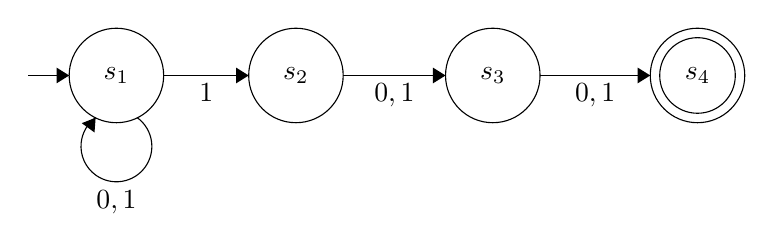
\begin{tikzpicture}[scale=0.2]
\tikzstyle{every node}+=[inner sep=0pt]
\draw [black] (5.8,-3.2) circle (3);
\draw (5.8,-3.2) node {$s_1$};
\draw [black] (17.2,-3.2) circle (3);
\draw (17.2,-3.2) node {$s_2$};
\draw [black] (29.7,-3.2) circle (3);
\draw (29.7,-3.2) node {$s_3$};
\draw [black] (42.7,-3.2) circle (3);
\draw (42.7,-3.2) node {$s_4$};
\draw [black] (42.7,-3.2) circle (2.4);
\draw [black] (0.2,-3.2) -- (2.8,-3.2);
\fill [black] (2.8,-3.2) -- (2,-2.7) -- (2,-3.7);
\draw [black] (8.8,-3.2) -- (14.2,-3.2);
\fill [black] (14.2,-3.2) -- (13.4,-2.7) -- (13.4,-3.7);
\draw (11.5,-3.7) node [below] {$1$};
\draw [black] (20.2,-3.2) -- (26.7,-3.2);
\fill [black] (26.7,-3.2) -- (25.9,-2.7) -- (25.9,-3.7);
\draw (23.45,-3.7) node [below] {$0,1$};
\draw [black] (32.7,-3.2) -- (39.7,-3.2);
\fill [black] (39.7,-3.2) -- (38.9,-2.7) -- (38.9,-3.7);
\draw (36.2,-3.7) node [below] {$0,1$};
\draw [black] (7.123,-5.88) arc (54:-234:2.25);
\draw (5.8,-10.45) node [below] {$0,1$};
\fill [black] (4.48,-5.88) -- (3.6,-6.23) -- (4.41,-6.82);
\end{tikzpicture}
\end{center}

\begin{tabular}{ll}
{\bf Def:} & A \underline{nondeterministic finite automata (NFA)} is a 5-tuple \\
& $N=(Q,\Sigma,\Delta,S,F)$ where \\
& $\cdot$ $Q,\Sigma,F$ are the same as in DFA \\
& $\cdot$ $S\subseteq Q$ is the set of start states \\
& $\cdot$ $\Delta : Q \times E \rightarrow P(Q)$ is the transition function \\ 
\\
{\bf Intuition:} & An NFA $N=(Q,\Sigma,\Delta,S,F)$ may start in any state in $S$. Like a DFA, \\
& it reads an input string $x\in\Sigma^*$ one symbol at a time. If it is in state $q$ at the \\
& time $t$ and reads $a\in\Sigma$, then at time $t+1$ it may be in any state $q'\in\Delta(q,a)$. \\
& \\
& "\underline{The magic:}" If there is some way for $N$ to accept, (proceedint as above) \\
& then it does so, and we say that $N$ accepts $x$, otherwise $N$ rejects $x$. \\
\\
{\bf Example:} & Design an NFA that accepts the language \\
& $A=\{x\in\{0,1\}^*$ s.t. $|x|$ is divisible by 3 or 5$\}$.
\end{tabular}

\begin{center}
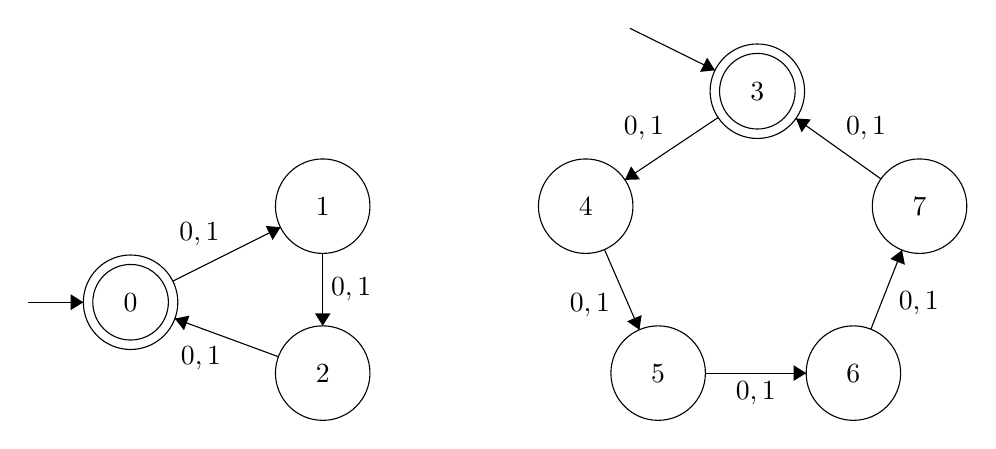
\begin{tikzpicture}[scale=0.2]
\tikzstyle{every node}+=[inner sep=0pt]
\draw [black] (6.7,-17.6) circle (3);
\draw (6.7,-17.6) node {$0$};
\draw [black] (6.7,-17.6) circle (2.4);
\draw [black] (18.9,-11.5) circle (3);
\draw (18.9,-11.5) node {$1$};
\draw [black] (18.9,-22.1) circle (3);
\draw (18.9,-22.1) node {$2$};
\draw [black] (35.6,-11.5) circle (3);
\draw (35.6,-11.5) node {$4$};
\draw [black] (40.2,-22.1) circle (3);
\draw (40.2,-22.1) node {$5$};
\draw [black] (52.6,-22.1) circle (3);
\draw (52.6,-22.1) node {$6$};
\draw [black] (56.8,-11.5) circle (3);
\draw (56.8,-11.5) node {$7$};
\draw [black] (46.5,-4.2) circle (3);
\draw (46.5,-4.2) node {$3$};
\draw [black] (46.5,-4.2) circle (2.4);
\draw [black] (36.79,-14.25) -- (39.01,-19.35);
\fill [black] (39.01,-19.35) -- (39.15,-18.42) -- (38.23,-18.81);
\draw (37.17,-17.77) node [left] {$0,1$};
\draw [black] (43.2,-22.1) -- (49.6,-22.1);
\fill [black] (49.6,-22.1) -- (48.8,-21.6) -- (48.8,-22.6);
\draw (46.4,-22.6) node [below] {$0,1$};
\draw [black] (53.71,-19.31) -- (55.69,-14.29);
\fill [black] (55.69,-14.29) -- (54.94,-14.85) -- (55.87,-15.22);
\draw (55.45,-17.67) node [right] {$0,1$};
\draw [black] (54.35,-9.77) -- (48.95,-5.93);
\fill [black] (48.95,-5.93) -- (49.31,-6.81) -- (49.89,-5.99);
\draw (53.4,-7.35) node [above] {$0,1$};
\draw [black] (44.01,-5.87) -- (38.09,-9.83);
\fill [black] (38.09,-9.83) -- (39.04,-9.8) -- (38.48,-8.97);
\draw (39.3,-7.35) node [above] {$0,1$};
\draw [black] (38.4,-0.2) -- (43.81,-2.87);
\fill [black] (43.81,-2.87) -- (43.31,-2.07) -- (42.87,-2.97);
\draw [black] (0.2,-17.6) -- (3.7,-17.6);
\fill [black] (3.7,-17.6) -- (2.9,-17.1) -- (2.9,-18.1);
\draw [black] (9.38,-16.26) -- (16.22,-12.84);
\fill [black] (16.22,-12.84) -- (15.28,-12.75) -- (15.72,-13.65);
\draw (11.07,-14.04) node [above] {$0,1$};
\draw [black] (18.9,-14.5) -- (18.9,-19.1);
\fill [black] (18.9,-19.1) -- (19.4,-18.3) -- (18.4,-18.3);
\draw (19.4,-16.8) node [right] {$0,1$};
\draw [black] (16.09,-21.06) -- (9.51,-18.64);
\fill [black] (9.51,-18.64) -- (10.09,-19.38) -- (10.44,-18.45);
\draw (11.17,-20.39) node [below] {$0,1$};
\end{tikzpicture}
\end{center}

$\textbf{Formal Semantics of NFAs:}$
\begin{itemize}
\item Let $N=(Q,\Sigma,\Delta,S,F)$ be an NFA. We define the \underline{extended transition function}: \\
$\hat{\Delta}:P(Q)\times\Sigma^*\rightarrow P(Q)$ as follows.
\item We want $\hat{\Delta}(A,x)$ to be the set of all states that are reachable from $A$ by processing $x$.
\item The definition of $\hat{\Delta}(A,x)$ is recursive. \\
$\hat{\Delta}(A,\lambda)=A$ \\
$\hat{\Delta}(A,xa)=\cup_{q\in\hat{\Delta}(A,x)}\Delta(q,a)$
\end{itemize}

\begin{tabular}{ll}
{\bf Def:} & An NFA $N$ \underline{accepts} a string $x\in\Sigma^*$ if $\hat{\Delta}(s,x)\cap F=\emptyset$, otherwise $N$ rejects $x$. \\
\\
{\bf Fact:} & For every DFA $M$, there is an NFA $N$ s.t. $L(M)=L(N)$ \\
\\
{\bf Theorem:} & For every NFA $N$, there is a DFA $M$ s.t. $L(M)=L(N)$. \\
\end{tabular}

\section{Grammar}

\begin{longtable}{ll}
{\bf Def:} & A sequence $S\in\{0,1\}^{\infty}$ is \underline{normal} if and only if no finite-state gambler can make \\
& unbounded money placing fair bets on it. \\
& $\therefore$ Normality is finite-state randomness.\\
\\
{\bf Def:} & A \underline{context-free-grammar} is a 4-tuple \\
& $G=(N,\Sigma,P,S)$ where \\
& $\cdot$ $N$ is an alphabet of \underline{non-terminal} symbols \\
& $\cdot$ $\Sigma$ is an alphabet of \underline{terminal} symbols \\
& $\cdot$ $N \cap \Sigma = \emptyset$ \\
& $\cdot$ $S\in\mathbb{N}$ is the start symbol \\
& $\cdot$ $P$ is a finite set of \underline{productions}, each of which is of the form $A\rightarrow \alpha$, where \\
& $A \in N$ and $\alpha\in(N\cup\Sigma)*$ \\
\\
{\bf Semantics:} & Let $G=(N,\Sigma,P,S)$ be a CFG. For $\alpha,\beta\in(N\cup\Sigma)^*$, we say that $\beta$ is \\
& \underline{derivable} from $\alpha$ in one step, and we write $\alpha\dfrac{\textcircled{1}}{G}\beta$. If there exists \\
& a production $A\rightarrow\gamma$ in $P$ and strings $\alpha_1,\alpha_2\in(N\cup\Sigma)^*$ such that \\ 
& $\alpha = \alpha_1A\alpha_2$ and $\beta=\alpha_1\gamma\alpha_2$. \\
& \\
& For each $n\in\mathbb{N}$, define the relation $\dfrac{n}{G}$ on $(N\cup\Sigma)^*$\\
& $\cdot$ $\alpha\dfrac{0}{G}\beta$ $\Leftrightarrow$ $\alpha = \beta$ \\
& $\cdot$ $\alpha\dfrac{n+1}{G}\beta$ $\Leftrightarrow$ $\exists\gamma\in(N\cup\Sigma)^*$ s.t. $\alpha\dfrac{n}{G}\gamma$ and $\gamma\dfrac{\textcircled{1}}{G}\beta$ \\
\\
{\bf Def:} & If $\alpha,\beta\in(N\cup\Sigma)^*$, then $\beta$ is \underline{derivable} from $\alpha$, and we write \\
& $\alpha\dfrac{*}{G}\beta$ if there exists $n\in\mathbb{N}$ s.t. $\alpha\dfrac{n}{G}\beta$. \\
\\
{\bf Def:} & The \underline{language} generated by $G$ is $L(G)=\{x\in\Sigma^*|S\dfrac{*}{G}x\}$ \\
\\
{\bf Def:} & A \underline{context-free-language} is a language $A\subseteq\Sigma^*$ for which there exists \\
& a CFG $G$ s.t. $L(G)=A$. \\
\\
{\bf Terminology:} & Let $G=(N,\Sigma,P,S)$ be a CFG. \\
& $\cdot$ a \underline{sequential form} of $G$ is a string $\alpha\in(N\cup\Sigma)^*$ s.t. $S\dfrac{*}{G}\alpha$ \\
& $\cdot$ a \underline{sentence} of $G$ is a terminal string $x\in\Sigma^*$ s.t. $S\dfrac{*}{G}x$ \\
\\
{\bf Def:} & A \underline{right-linear grammar} is a CFG all of whose productions are of the form \\
& $A \rightarrow xB$ or $A\rightarrow x$ where $A,B\in N$ and $x\in\Sigma^*$. \\
\\
{\bf Def:} & A \underline{strongly right-linear grammar} is a right-linear grammar, all of whose \\
& productions are of the form $A\rightarrow aB$ or $A \rightarrow\lambda$, where $A,B\in N$ and $a\in\Sigma$. 
\end{longtable}

\end{document}